%%%%%%%%%%%%%%%%%%%%%%%%%%%%%%%%%%%%%%%%%%%%%%%%%%%%%%%%%%%%%%%
%
% Welcome to Overleaf --- just edit your LaTeX on the left,
% and we'll compile it for you on the right. If you open the
% 'Share' menu, you can invite other users to edit at the same
% time. See www.overleaf.com/learn for more info. Enjoy!
%
%%%%%%%%%%%%%%%%%%%%%%%%%%%%%%%%%%%%%%%%%%%%%%%%%%%%%%%%%%%%%%%
\documentclass{beamer}
\usepackage[utf8]{inputenc}
\usepackage{xeCJK}
\usepackage{graphics}
\usepackage{caption}
\usepackage{subfigure}
\usepackage{listings}
\usepackage{xcolor}

\usetheme{Madrid}
\usecolortheme{default}

%----------------------------导言区--------------------------------
%This block of code defines the information to appear in the
%Title page
\title[|复杂系统|] %optional
{《复杂系统》}
\usepackage{ctex} 

\subtitle{Figure : 4.8/5.1/5.2/5.3}

\author[指导老师:王瑞琦] % (optional)
{}

\institute[SHU] % (optional)
{
  \Large{\begin{block}{\centerline{\large{Shanghai University}}}
  \centerline{\small{College of Sciences-Department of Mathematics}}
  \end{block}}
  \and
  \large{Jie Xing}-\normalsize{Information and Computing Sciences}\\
  \large{Haitao Yan}-\normalsize{Mathematics and Applied Mathematics}\\
  \large{Zhihao Gu}-\normalsize{Mathematics and Applied Mathematics}\\
}

\date[2022-3-29] % (optional)
{Mar.29, 2022}

\logo{
\includegraphics[height=1cm]{SHU}}

%End of title page configuration block
%------------------------------------------------------------



%------------------------------------------------------------
%The next block of commands puts the table of contents at the 
%beginning of each section and highlights the current section:

\AtBeginSection[]
{
  \begin{frame}
    \frametitle{目录\songti}
    \tableofcontents[currentsection]
  \end{frame}
}
%------------------------------------------------------------


\begin{document}

%The next statement creates the title page.
\frame{\titlepage}


%---------------------------------------------------------
%This block of code is for the table of contents after
%the title page
\begin{frame}
\frametitle{目录}
\tableofcontents
\end{frame}
%---------------------------------------------------------

\section{Mathematical modeling}
     \begin{frame}
      \frametitle{Model Analysis \uppercase\expandafter{\romannumeral1}}
      
      %\pause

      \begin{itemize}
       \item 人口增长模型:
        \begin{block}{}
		 \begin{equation*}
		  \begin{aligned}
			x_t&=ax_{t-1}
		  \end{aligned}
		 \end{equation*}
        \end{block}
       \item 满足两个条件
        \begin{itemize}
				\item 指数增长
				\item 收敛到一定的极限
			\end{itemize}
	   \item 用$f(x_{t-1})$来代替a
	    \begin{block}{}
		 \begin{equation*}
		  \begin{aligned}
			x_t&=f(x_{t-1})x_{t-1} 
		  \end{aligned}
		 \end{equation*}
        \end{block}
       \item 函数f(x)需要经过(x,f(x))=(0,a)和(K,1)两点。 
	   
       \end{itemize}
     \end{frame}

%--------------------------
\begin{frame}{Model Analysis \uppercase\expandafter{\romannumeral1}}
 \begin{itemize}
     \item 用线性函数表示f(x)
      \begin{block}{}
		 \begin{equation*}
		  \begin{aligned}
			f(x)&=-\frac{a-1}{K}x+a \\
			x_t&=(-\frac{a-1}{K}x_{t-1}+a)x_{t-1} 
		  \end{aligned}
		 \end{equation*}
        \end{block}
        这就是$Logistic$模型
     \item 令$r=a-1$,则
      \begin{block}{}
		 \begin{equation*}
		  \begin{aligned}
			x_t&=(-\frac{a-1}{K}x_{t-1}+a)x_{t-1}\\ 
			&=(-\frac{r}{K}x_{t-1}+r+1)x_{t-1}\\
			&=x_{t-1}+rx_{t-1}(1-\frac{x_{t-1}}{K})
		  \end{aligned}
		 \end{equation*}
        \end{block}
 \end{itemize}
\end{frame}

\begin{frame}{Model Analysis \uppercase\expandafter{\romannumeral1}}
 \begin{itemize}
     \item 如果x远小于K
      \begin{block}{}
		 \begin{equation*}
		  \begin{aligned}
			x_t&\approx x_{t-1}+rx_{t-1}
		  \end{aligned}
		 \end{equation*}
        \end{block}
        以上就是单变量的模型建立
 \end{itemize}
\end{frame}

\begin{frame}{Model Analysis \uppercase\expandafter{\romannumeral2}}
 \begin{itemize}
     \item 考虑一个典型场景——捕食者(y)与猎物(x)两个种群间相互作用\\
     根据一维的$Logistic$模型和指数衰减模型,分别针对猎物和捕食者建立同样的数学模型,将假设所得出的函数代入方程,可以得到
      \begin{block}{}
		 \begin{equation*}
		  \begin{aligned}
			x_t&=x_{t-1}+rx_{t-1}(1-\frac{x_{t-1}}{K})-(1-\frac{1}{by_{t-1}+1})\\
			y_t&=y_{t-1}-dy_{t-1}+cx_{t-1}y_{t-1}
		  \end{aligned}
		 \end{equation*}
        \end{block}
 \end{itemize}
\end{frame}





%---------------------------------------------------------

\section{4.8-Simulation results of the predator-prey model}
    \begin{frame}
     \frametitle{4.8}
      Building Your Own Model Equations with Multiple Variables\\
      ~\\令$r=b=d=c=1,K=5,x_0=y_0=1$\\
      此时的捕食者-猎物模型的模拟结果如下图(\ref{fig1}):\\

    \begin{figure}
		\centering
		 \subfigure[State variables plotted over time]{
		  \label{fig:subfig:a}             %% label for first subfigure
		   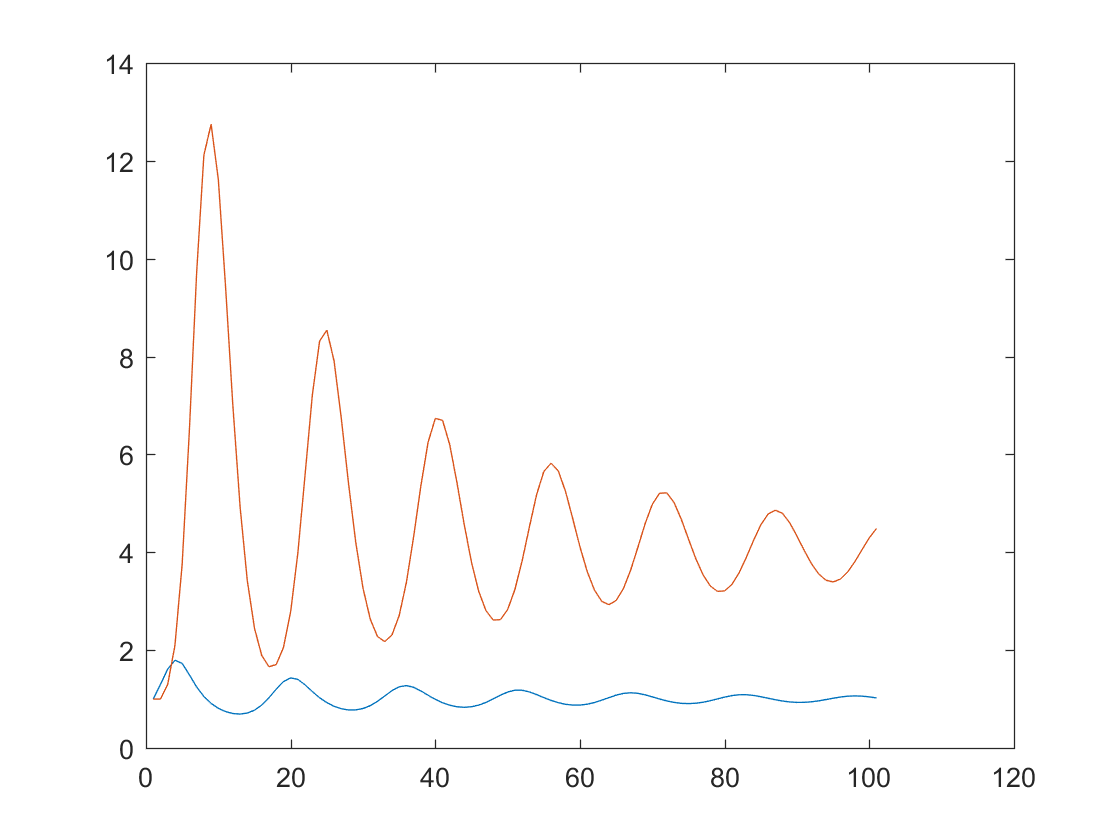
\includegraphics[width=1.6in]{p1}}
		\hspace{0.4in}
		 \subfigure[ Phase space visualization of the same result]{
		  \label{b}                       %% label for second subfigure
			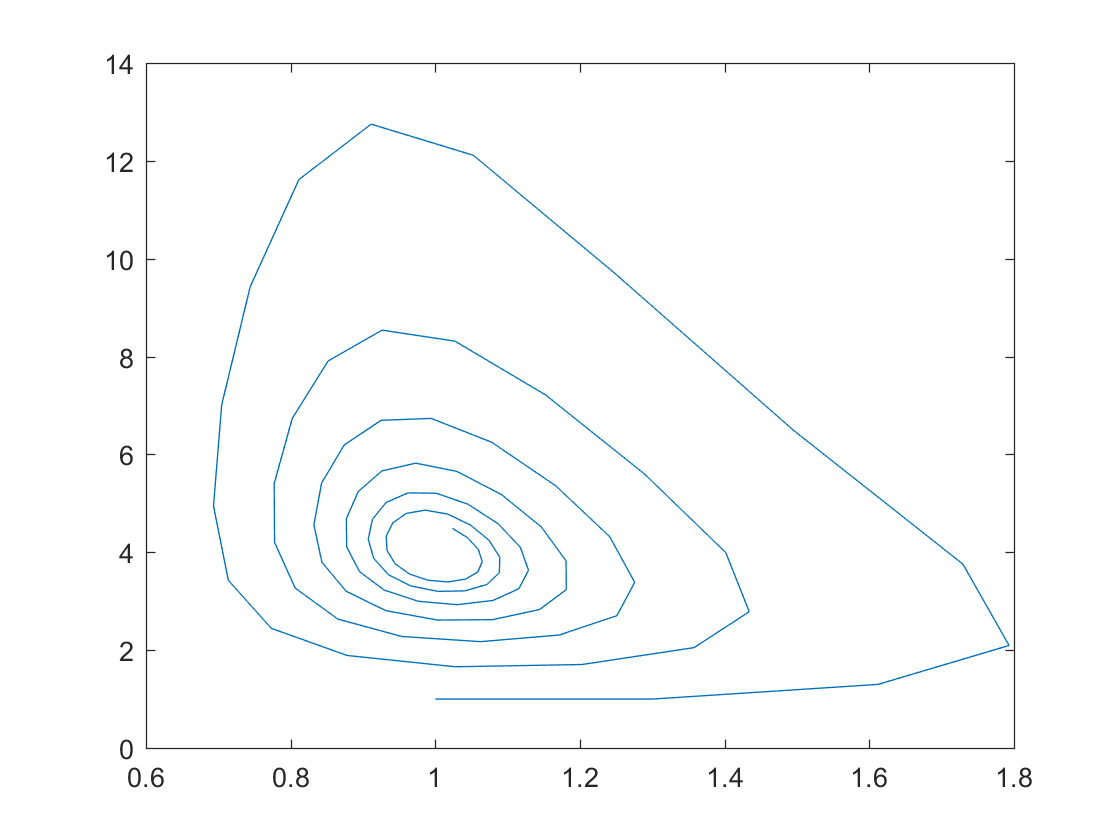
\includegraphics[width=1.6in]{p2}}
		\caption{Simulation results of the predator-prey mode}
		\label{fig1}                      %% label for entire figure
	\end{figure}
\end{frame}

%~~~~~~~~~~~~~~~~~~~~~~~~~~~~~~~~~~~~~~~~~~~~~~~~
%New colors defined below
\definecolor{codegreen}{rgb}{0,0.6,0}
\definecolor{codegray}{rgb}{0.5,0.5,0.5}
\definecolor{codepurple}{rgb}{0.58,0,0.82}
\definecolor{backcolour}{rgb}{0.95,0.95,0.92}

%Code listing style named "mystyle"
\lstdefinestyle{mystyle}{
  backgroundcolor=\color{backcolour},   commentstyle=\color{codegreen},
  keywordstyle=\color{magenta},
  numberstyle=\tiny\color{codegray},
  stringstyle=\color{codepurple},
  basicstyle=\ttfamily\footnotesize,
  breakatwhitespace=false,         
  breaklines=true,                 
  captionpos=b,                    
  keepspaces=true,                 
  numbers=left,                    
  numbersep=3pt,                  
  showspaces=false,                
  showstringspaces=false,
  showtabs=false,                  
  tabsize=1
}


\begin{frame}[fragile]{Matlab for 4.8 Left}
 \begin{lstlisting}[language=Matlab ,style=mystyle]
r=1;
b=1;
c=1;
d=1;
s=100;
X=zeros(1,s);                                                         
Y=zeros(1,s);
X(1,1)=1;                                                             
Y(1,1)=1;
for t=1:1:100
    X(1,t+1)=X(1,t)+X(1,t).*(r-1+1./(b.*Y(1,t)+1)-X(1,t)./5);
    Y(1,t+1)=(1-d).*Y(1,t)+c.*Y(1,t).*X(1,t);
end
plot(X)
hold on
plot(Y)
hold off
\end{lstlisting}
\end{frame}

\begin{frame}[fragile]{Matlab for 4.8 Right}
 \begin{lstlisting}[language=Matlab ,style=mystyle]
r=1;
b=1;
c=1;
d=1;
s=100;
X=zeros(1,s);
Y=zeros(1,s);
X(1,1)=1;
Y(1,1)=1;
for t=1:1:100
    X(1,t+1)=X(1,t)+X(1,t).*(r-1+1./(b.*Y(1,t)+1)-X(1,t)./5);
    Y(1,t+1)=(1-d).*Y(1,t)+c.*Y(1,t).*X(1,t);
end
plot(X,Y);
\end{lstlisting}
\end{frame}


%---------------------------------------------------------

\section{5.1-Phase space drawn}
     \begin{frame}[fragile]
      \frametitle{绘制相空间}
\begin{alertblock}{Matlab for 5.1}
\begin{lstlisting}[language=Matlab ,style=mystyle]
s=30;
X=zeros(1,s);
Y=zeros(1,s);
for x0=-2:0.5:2
    for y0=-2:0.5:2
        X(1,1)=x0;
        Y(1,1)=y0;
        for t=1:s
            X(1,t+1)=0.5.*X(1,t)+Y(1,t);
            Y(1,t+1)=-0.5.*X(1,t)+Y(1,t);
        end
        plot(X,Y)
        hold on;
    end
end
hold off;
\end{lstlisting}
\end{alertblock}

\end{frame}




%---------------------------------------------------------

\section{5.2-Three-dimensional phase space drawn}
     \begin{frame}[fragile]
      \frametitle{绘制三维相空间}
      Matlab for 5.2
\begin{lstlisting}[language=Matlab ,style=mystyle]
s=30;
X=zeros(1,s);Y=zeros(1,s);Z=zeros(1,s);
for x0=-2:1:2
    for y0=-2:1:2
        for z0=-2:1:2
        X(1,1)=x0;
        Y(1,1)=y0;
        Z(1,1)=z0;
        for t=1:s
            X(1,t+1)=0.5.*X(1,t)+Y(1,t);
            Y(1,t+1)=-0.5.*X(1,t)+Y(1,t);
            Z(1,t+1)=-1*X(1,t)+(-1)*Y(1,t)+Z(1,t);
        end
        plot3(X,Y,Z)
        hold on;
        end
    end
end
hold off;
\end{lstlisting} 
\end{frame}


%---------------------------------------------------------

\section{5.3-Phase bad space drawn}
     \begin{frame}[fragile]
      \frametitle{轨迹相互交叉的离散时间模型相空间}
       \begin{alertblock}{Matlab for 5.3}
\begin{lstlisting}[language=Matlab ,style=mystyle]
s=30;
X=zeros(1,s);
Y=zeros(1,s);
for x0=-2:0.5:2
    for y0=-2:0.5:2
        X(1,1)=x0;
        Y(1,1)=y0;
        for t=1:s
            X(1,t+1)=-0.5.*X(1,t)+-0.7.*Y(1,t);
            Y(1,t+1)=X(1,t)+-0.5.*Y(1,t);
        end
        plot(X,Y)
        hold on;
    end
end
hold off;
\end{lstlisting}
\end{alertblock}
     \end{frame}

%---------------------------------------------------------
\begin{frame}{}
\begin{block}{}
\centerline{\huge{\itshape\ttfamily{Thanks for your Listening!}}}
\end{block}
\end{frame}


%---------------------------------------------------------

\end{document}